\documentclass{article}
\usepackage{listings}
\usepackage{graphicx}
\usepackage{float}
 
\floatstyle{ruled}
\newfloat{program}{thp}{lop}
\floatname{program}{Snippet}


\begin{document}

\title{Project Report - Limited Static Type Checking for JavaScript}
\author{Huascar A. Sanchez \and Tim Disney}

\maketitle

\lstset{showstringspaces=false}

\section{Introduction}
It is well known that in the construction of software it is generally cheaper to 
catch programming errors earlier in the development cycle \cite{cc2}. One method 
of catching these errors is static type checking. As we all know with static type 
checking, the type consistency of your code will be checked before the program is 
run. In other words, if there are any type violation in your code the the type 
checker will catch it. 

For example, invoking a method on an object that does not support it will be easily 
detected in strongly typed languages like Java. The compiler will immediately 
complain and will prevent the program from running. However, in languages like 
JavaScript, this type of error will be overlooked and deffered until runtime.

Enabling static type checking in a language as dynamic as JavaScript is a 
challenge. Especially since types can be modified at runtime. Given this constraint, 
we implemented a static type checker, called JSCheck, for prototype based objects 
in JavaScript. The scope of our checker was limited to properties on objects' 
prototype. In other words, we are completely ignoring type checking of things 
like strings and numbers. The whole idea, as Lucas Cardelli said \cite{typesystems}, 
is to prevent the occurance of execution errors during the running of your program. 

Our implementation is both unsound and incomplete. One thing that sets our 
implementation apart for previous work is that our checker works (in a limited 
fashion) for full JavaScript.

The rest of this paper is divided as follows. The implementation section will discuss 
any design and implementation choices that were made throughout the development 
of this static type checker. A collection of snippets is provided to show our checker 
in action. Our findings and conclusions will be discussed in the last section of 
this paper.


\section{Types in JavaScript}
\label{sec:types}
User defied types in JavaScript can be written in a variety of styles. The style
that we have focused on for the scope of this project was constructor functions and
adding fields to the type's prototype.

\begin{program}
\begin{verbatim}
function Dog(){
  // ..
}

Dog.prototype.getName = function(){
  //..
}

Dog.prototype.bark = function(){
  //..
}
\end{verbatim}
\caption{Checking Types in JavaScript}
\label{fig:object}
\end{program}

In the JavaScript code snippet (\ref{fig:object}) we define a {\tt Dog} type
which has two methods, {\tt getName} and {\tt bark} which are added to the {\tt Dog}
prototype.

There are other ways of creating objects including using object literal notation
or assigning methods directly to fields of the object but these techniques of 
object creation are not included in the scope what JSCheck will recognize.

To enable JSCheck to check type usages we add the comment type annotation
format to the JavaScript language as seen in snippet \ref{fig:check}. In
this example the {\tt fido} parameter has been annotated with the {\tt Dog}
type in the {\tt //\#} comment. JSCheck will then check that all usages of
the {\tt fido} parameter conforms to the definition of the {\tt Dog} type.

\begin{program}
\begin{verbatim}
//# @type Dog fido
function useDog(fido) {
  fido.bark();
}

var d = new Dog();
useDog(d);
\end{verbatim}
\caption{Type Checking}
\label{fig:check}
\end{program}


\section{Implementation}
\label{sec:implementation}
JSCheck is implemented in Haskell. We were originally considering defining a 
subset of JavaScript to easy the burden of creating a parser for JavaScript. 
However we found a Haskell library called HJS \cite{hjsLibrary} 
which already implements a full parser for JavaScript (ECMAScript 3rd edition plus 
some additions from JavaScript 1.5). We had to make a few modifications to
HJS in order to pick up the type annotations but but this was a huge win
in terms of effort for features.

As seen in figure \ref{fig:jscheckway} In general terms JSCheck works by taking in a JavaScript source file and running
a modified version of the HJS parser over it. This produces a abstract syntax tree
that is fed into a type extractor function which finds all the JavaScript object types that
has been defined in the source. The output of this function is a list of types (type names and all associated fields)
which is fed into a type checker function along with the original AST. The
checker function find all functions that have been annotated with our special
type comments and checks all usages of parameters against the extracted types. 
If there are any usages of unknown fields the checker fails with a warning that
the source could not be checked.

Because of the dynamic nature of JavaScript our implementation is both unsound 
and incomplete. It is unsound because methods could be add to the object at
runtime so even though the checker sees a usage of an unknown field that field
actually could be defined. It is incomplete because fields could also be removed
from an object at runtime. The JavaScript program could be accessing non existent 
fields even though the checker thought they were there.

Unless you explicity type annotate your functions, JScheck does not have the means 
for type checking them. The way our checker works is very straightforward. It a
three-steps process (see Figure ~\ref{fig:jscheckway}). First, it takes some JavaScript 
code and parses it. The output is an Abstract Syntax Tree (AST). Second, given this AST, 
it extracts all the possible types found in your code. The output is what we know 
as the environment. The environment is the place where type names are mapped to 
their available type fields. Third, the environment and the AST are then fed to 
a built-in type checking process. Here is where any type consistency will be checked 
and, if there are any, type consistency violations will be communicated to the 
developer. 

\begin{figure}[here]
  \begin{center}
    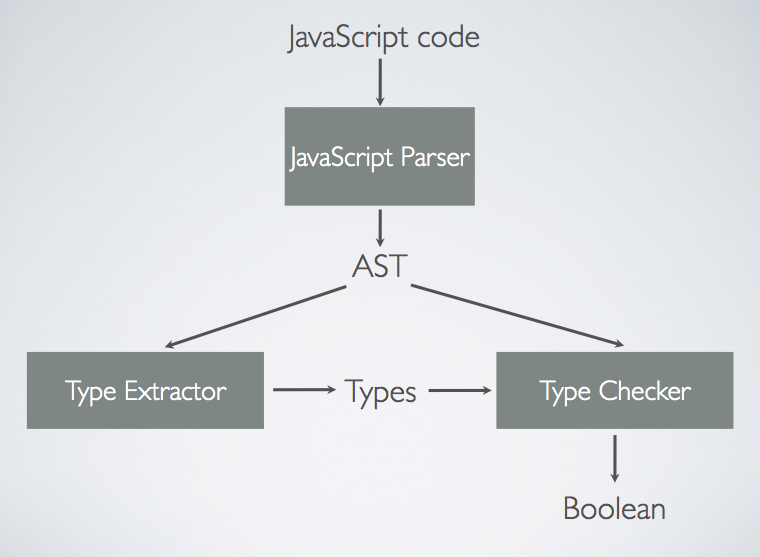
\includegraphics[scale=0.5]{blockdiagram.png}
  \end{center}
  \caption{Type Checking - the JSCheck way}
  \label{fig:jscheckway}
\end{figure}
\pagebreak



As could see in the above figure, after the code has been parsed, the JScheck will 
extract the types and check them on functions that have type annotations. The final 
output will be either your code is well-typed or not (represented as a boolean value). 
We plan on changing this output to a more descriptive one (i.e., including where the
type violation occurred, the name of the function, and a suggestion for how to fix it). 


\section{Related Work}
We are not the first ones who have tried to implement static type checking for JavaScript.
There have been others who have done it before us. Some of them include:

\begin{description}
  \item[Tom Austin and Caitlin Sadowski] \hfill \\ 
  developed a structural type-checker for Javascript \cite{fwjsStruct}.
  \item[$JS_0$ team] \hfill \\ 
  developed a formalism for an object based language called JSO, which includes features of JavaScript 
  \cite{typeinferenceforjavascriptEcoop,typecheckingforjavascript}. 
  \item[DRuby team] \hfill \\ 
  developed Diamondback Ruby (DRuby), a tool that blends Ruby's dynamic type 
  system with a static typing discipline \cite{typecheckingruby}.
  \item[Google] developed the Closure compiler \cite{closureCompiler}.  
\end{description}

In some way, which remains obscure, we all shared the same drive for making type 
checking possible in a dynamic language. We chose JavaScript for many reasons. 
However, the most important one, for us, was that JavaScript is the most used 
language in the World Wide Web and providing this type checking capability would
be appreciated by many. 

\section{Future Work}
There are several areas in our static type checker that could be expanded. One of
them, as indicated above, is the type checking output. Future will be focused on 
providing a more descriptive type checking output. Another extension could be to
provide type consistency checks for other elements of the language, like strings
and numbers.


One thing that sets our 
implementation apart for previous work is that our checker works (in a limited fashion) for
full JavaScript.

\section{Conclusion}
\label{sec:conclusion}
We have developed a static type checker for prototype based objects in JavaScript
called JSCheck. By using this checker any developer will be able to catch any 
type errors before running their programs. The only thing the developer needs to
do is to explicitly type annotate a function(s). The rest is done by JSCheck. 

The idea of implementing a type checker strongly motivated us. It is hard for us 
describe the feeling of accomplishment after completing our implementation. Now,
for sure, we have a better understanding of what static type checking is all about. 

Full source can be found at {\tt http://github.com/disnet/jscheck}.

\bibliographystyle{abbrv}
\bibliography{report}

\end{document}


